\chapter{What Is Meditation?}

This chapter follows J. Krishnamurti's San Diego 1970 inquiry into meditation, with source credit to J. Krishnamurti and the Krishnamurti Foundation Trust, and curation for \emph{How You Got Happiness?} by LazyingArt LLC through Video2Book. The talk belongs in the third part of the book because it does not offer meditation as a method for becoming happy. It asks what must end before meditation can be understood: search, image, recognition, control, method, experience, and the whole habit of moving away from what is.

\section{Before Asking What Meditation Is}

Krishnamurti begins by delaying the question. We are going to ask what meditation is, but we cannot ask that question directly if meditation has already become another object to obtain. So the first question is not ``How shall we meditate?'' but ``What are we after?''

That delay is the first mathematical move of the chapter, if we use the word mathematical in the broad sense of tracking structure. A search is not innocent. To seek truth, God, a perfect life, hope, or companionship is already to carry some contour of what is sought. The mind may not have a precise definition, but it has an image, a pattern, an idea, a recognizable form. Otherwise it would not know that it had found what it was seeking.

We can record the structure as follows:
\begin{equation}
\mathrm{Search}
\longrightarrow
\mathrm{Image}
\longrightarrow
\mathrm{Recognition}
\longrightarrow
\mathrm{AlreadyKnown}.
\end{equation}

This notation is only a compact companion to the lecture. It is not a psychological model. Its point is simple: recognition implies previous knowledge. Therefore a search that depends on recognition remains inside the field of the already known.

\begin{proposition}
If meditation is approached as a search for a predetermined object, it is already shaped by desire, image, and recognition.
\end{proposition}

\begin{proof}
To search is to be able, at least vaguely, to recognize the object sought. Recognition presupposes some prior image, memory, or contour. Therefore the sought object is measured by what the mind already carries. In that case meditation has become another movement toward the known, not an inquiry into the unknown.
\end{proof}

The first negative statement is therefore severe:
\begin{equation}
\mathrm{Meditation} \Rightarrow \neg \mathrm{Search}.
\end{equation}

Every form of search must come to an end, not because seeking is morally blameworthy, but because seeking has already projected the object it hopes to discover. If one is unhappy or lonely, one may seek hope or companionship and inevitably find some sustaining image. But meditation, as this talk approaches it, cannot be another search for consolation.

\section{Order Without Blueprint}

The next movement is still not a definition of meditation. Krishnamurti says a foundation must be laid. The foundation is order, or virtue, but he immediately separates it from respectability and from social morality. Order is not conformity to a public standard. It is not produced by authority, by a private blueprint, or by one's own accumulated experience.

The lecture's positive relation is:
\begin{equation}
\mathrm{Understanding}(\mathrm{Disorder}) \longrightarrow \mathrm{Order}.
\end{equation}

The rejected relation is:
\begin{equation}
\mathrm{Order} \neq
f(\mathrm{Blueprint},\mathrm{Authority},\mathrm{Experience},\mathrm{Effort}).
\end{equation}

Disorder exists as long as there is conflict, both outwardly and inwardly. Therefore order cannot be imposed by effort, because effort belongs to the same field of conflict. We are not adding a better control. We are asking whether disorder can be understood without the movement that distorts it.

\subsection{Question \& Answer}

\paragraph{Question.}
How can order come about without control?

\paragraph{Answer.}
It comes about only through understanding disorder. That means observing conflict as it is, without suppressing it, overcoming it, throttling it, justifying it, or choosing for or against it. The difficulty is that we usually meet disorder with effort, and effort, in this lecture, is already a distortion.

The local derivation is:
\begin{align}
\mathrm{Effort} &\longrightarrow \mathrm{Distortion},\\
\mathrm{Observation\ of\ Disorder} &\longrightarrow \mathrm{Understanding},\\
\mathrm{Understanding} &\longrightarrow \mathrm{Order}.
\end{align}

\begin{figure}
\centering
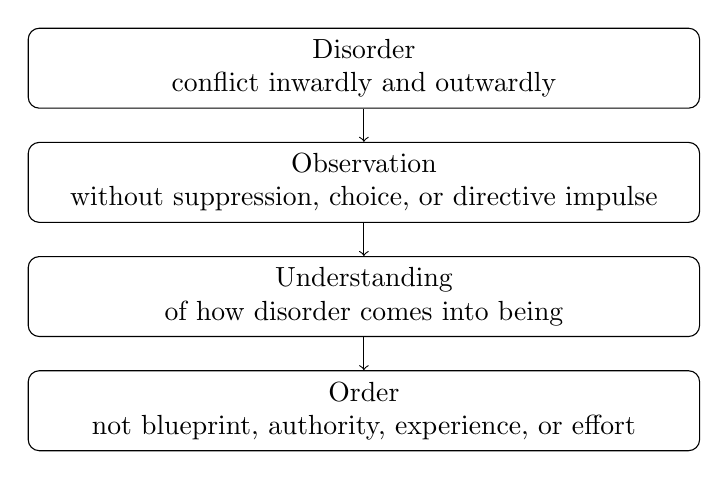
\begin{tikzpicture}[
  every node/.style={draw, rounded corners, align=center, text width=0.68\linewidth, inner sep=4pt},
  every path/.style={->}
]
\node (disorder) at (0,0) {Disorder\\conflict inwardly and outwardly};
\node (observe) at (0,-1.45) {Observation\\without suppression, choice, or directive impulse};
\node (understand) at (0,-2.90) {Understanding\\of how disorder comes into being};
\node (order) at (0,-4.35) {Order\\not blueprint, authority, experience, or effort};
\draw (disorder) -- (observe);
\draw (observe) -- (understand);
\draw (understand) -- (order);
\end{tikzpicture}
\caption{The lecture's movement from disorder to order, reconstructed as a narrow flow for pocket-size reading.}
\end{figure}

\section{The Controller Is The Controlled}

The ordinary answer to disorder is control. Krishnamurti now turns that answer inside out. Control implies suppression, rejection, exclusion, or a division between the one who controls and the thing to be controlled. Once that division appears, conflict appears with it.

The chain is:
\begin{equation}
\mathrm{Control}
\longrightarrow
(\mathrm{Controller}/\mathrm{Controlled})
\longrightarrow
\mathrm{Division}
\longrightarrow
\mathrm{Conflict}
\longrightarrow
\mathrm{Distortion}.
\end{equation}

This is why control cannot be the foundation of meditation. It reproduces the disorder it tries to master. The more subtle claim is that the controller is not actually separate from the controlled. The one who says, ``I am angry and I must get rid of anger,'' is not apart from anger. The division is part of anger's movement.

Krishnamurti's identity claim can be recorded compactly:
\begin{equation}
\mathrm{Controller}=\mathrm{Controlled},
\qquad
\mathrm{Observer}=\mathrm{Observed}.
\end{equation}

These equalities are not algebraic identities. They are inquiry-identities: markers for the collapse of a false inward separation. If the observer divides himself from anger, jealousy, despair, or the desire to fulfil, contradiction begins. Where there is contradiction, there is conflict. Where there is conflict, there is distortion.

\begin{remark}
This identity is the hinge of the foundation. Without seeing it, meditation easily becomes self-hypnosis: one fragment of the mind controlling another fragment and calling the struggle spiritual discipline.
\end{remark}

\section{Love, Learning, And Standing Alone}

The foundation now widens. Order alone is not enough if the mind is loveless. Krishnamurti introduces love through negation. Love is not sentiment, not romantic projection, not competition, and not the pursuit of pleasure. It is not divided into ``my love'' and ``your love.''

The relation is best kept negative:
\begin{equation}
\mathrm{Love}
\neq
g(\mathrm{Pleasure},\mathrm{Desire},\mathrm{Jealousy},\mathrm{Competition},\mathrm{Sentiment}).
\end{equation}

This is also why the talk pauses over discipline. Discipline is not obedience to another. It is learning. And learning, here, means observing oneself: self-centred activity, the tricks of the mind, images, illusions, delusions, sentimentality, and the movement of ``me'' and ``not me.'' Observation is not possible if we look through a conclusion, a prejudice, a formula, or the authority of a teacher.

So awareness cannot be handed down. We can be taught words, systems, postures, and practices; but Krishnamurti asks for a mind that stands alone, unburdened by propaganda and by the experiences of others. This is not a side complaint about organizations. It prepares the next rejection: no method can supply meditation.

\section{Observation, Exploration, And Experience}

The middle of the lecture makes several careful distinctions. Observation is not exploration. Exploration, in this context, involves analysis. Analysis implies an analyser and the thing analysed. Exploration implies an explorer. In each case, a center is acquiring and accumulating.

Observation is different. It is continuous learning, not continuous accumulation.

\begin{align}
\mathrm{Observation} &\longrightarrow \mathrm{Learning},\\
\mathrm{Exploration} &\longrightarrow \mathrm{Accumulation}
\longrightarrow \mathrm{Action\ from\ Accumulation}.
\end{align}

This distinction should not be flattened into an attack on reason. Krishnamurti allows that enquiry may be logical, sane, rational, and critical. But observation, as the lecture uses the word, is not the same as building a store of knowledge from which the self later acts.

\subsection{Question \& Answer}

\paragraph{Question.}
Why do we want deeper and wider experiences?

\paragraph{Answer.}
Because ordinary life often feels small, petty, fearful, and burdened. The craving for marvellous experience can become an escape from what is. But experience requires recognition. If we know an experience as pleasant, noble, mystical, spiritual, or beautiful, then recognition has already entered. Recognition belongs to the past.

The derivation is:
\begin{enumerate}
\item Experience must be recognized as experience.
\item Recognition depends on what is already known.
\item What is already known belongs to the past.
\item Therefore experience, as recognized experience, is not wholly new.
\item The craving for greater experience may become an escape from what is.
\end{enumerate}

In compact form:
\begin{equation}
\mathrm{Experience}
\longrightarrow
\mathrm{Recognition}
\longrightarrow
\mathrm{Past}.
\end{equation}

And:
\begin{equation}
\mathrm{Craving\ for\ Experience}
\longrightarrow
\mathrm{Escape\ from\ What\ Is}.
\end{equation}

This is why the talk can return to meditation only after method, purpose, search, hope, and experience have been put aside. Otherwise meditation becomes another refined appetite.

\section{Meditation Without Method}

Now the original question returns with more force: what is meditation? Krishnamurti refuses the familiar answer. Meditation is not sitting for a few minutes, fixing the mind on an image, repeating a formula, or battling to control thought. Any system soon becomes repetitive and mechanical. If we practise a method, we become what the method offers; and what a method offers is not truth, because truth is living while method is mechanical.

The old structure of division reappears:
\begin{equation}
\mathrm{Method}
\longrightarrow
\mathrm{Practice}
\longrightarrow
(\mathrm{Practitioner}/\mathrm{Practised})
\longrightarrow
\mathrm{Division}
\longrightarrow
\mathrm{Conflict}
\longrightarrow
\mathrm{Disorder}.
\end{equation}

The important point is repetition of form. The same division that made control disorderly also makes practice disorderly when practice is treated as a path to truth.

So what is the positive movement? The mind that observes must be quiet. Not quiet because it has been forced into silence, but quiet because clear seeing requires quietness. If we are to listen completely, we cannot at the same time translate, compare, condemn, judge, or drift elsewhere.

\begin{equation}
\mathrm{Necessity\ to\ See\ Clearly}
\longrightarrow
\mathrm{Quiet\ Mind}.
\end{equation}

This is the opposite of cultivating silence in time. To cultivate a still mind introduces the cultivator, the goal, and the interval between them. That is the old duality in a more delicate costume.

\subsection{Question \& Answer}

\paragraph{Question.}
If attention is not practised, what happens when the mind wanders?

\paragraph{Answer.}
We do not battle with wandering. We know inattention as inattention. The very awareness of inattention is attention. But if action comes out of that inattention, that action too must be seen.

A compact rule, not a technique, is:
\begin{align}
\mathrm{Practice}(\mathrm{Attention}) &\longrightarrow \mathrm{Inattention},\\
\mathrm{Awareness}(\mathrm{Inattention}) &\longrightarrow \mathrm{Attention}.
\end{align}

This looks like an update rule, but it is not offered as one. The point is not to perform a procedure. The point is to see, without battle and without choice, the movement that is actually taking place.

\section{The Still Body, Joy, And Attention In Sleep}

Silence of mind is not isolated from the body. Krishnamurti extends the inquiry to the organism: fidgeting, restless movement, bodily insensitivity, compulsion, overindulgence, and the dulling action of pleasure. The body, he says, has its own intelligence, which thought spoils when it pursues pleasure or forces the organism.

This should be read as part of the lecture's inquiry, not as medical instruction. The claim is inward and practical: a sensitive body, a quiet mind, and love without pleasure-distortion belong together.

\begin{equation}
\mathrm{Still\ Body}
+
\mathrm{Quiet\ Mind}
+
\mathrm{Love\ without\ Pleasure\text{-}Distortion}
\longrightarrow
\mathrm{Harmony}.
\end{equation}

Pleasure and joy are then distinguished:
\begin{align}
\mathrm{Pleasure} &\longrightarrow \mathrm{Motive},\\
\mathrm{Joy} &\longrightarrow \neg \mathrm{Motive}.
\end{align}

Joy cannot be held by declaring, ``I am joyous.'' The moment one seeks its cause in order to repeat it, it is no longer joy in the sense intended here. This distinction feeds back into the earlier rejection of search: the search for repeated joy turns joy into pleasure.

\subsection{Question \& Answer}

\paragraph{Question.}
What is the point of such a life?

\paragraph{Answer.}
Krishnamurti answers by questioning the one who asks. If the question comes as a demand for usefulness, then this kind of life has no point in that market of utility. But if this harmony is actually alive, then it is not a means to something else. It is everything: teacher, disciple, neighbour, cloud, beauty, and love are no longer divided in the old way.

The final movement concerns sleep. The waking mind, with all its daily activity, usually continues in sleep. Dreams are treated here as the continuation of the same movement: action, anxiety, fear, guilt, interpretation, and self-centred activity. But if thought is watched during the day, then sleep is not merely the continuation of unattended disorder.

\begin{equation}
\mathrm{Attention}_{\mathrm{day}}
\longrightarrow
\mathrm{Attention}_{\mathrm{sleep}}
\longrightarrow
\mathrm{Whole\ Mind\ Awake}.
\end{equation}

This should not be turned into sleep science. It is the lecture's final extension of attention. Attention is not only a waking discipline; when the mind is attentive during the day, Krishnamurti says there is attention in sleep.

Beyond that point the lecture refuses description. Every form of description is not the described:
\begin{equation}
\mathrm{Description} \neq \mathrm{Described}.
\end{equation}

One can point to the door. One cannot describe what is beyond it and remain faithful to the inquiry.

\section{Summary}

The lecture does not define meditation by offering a method. It approaches meditation by clearing away what meditation is not: search, predetermined image, hope as escape, imposed order, control, authority, practice, accumulated experience, and cultivated silence. The structure is negative, but not empty. Through negation it uncovers a precise movement: observe disorder without distortion; see the controller as the controlled and the observer as the observed; distinguish observation from exploration and experience; listen without translation; know inattention without battle; allow quietness to arise from the necessity of seeing clearly.

Meditation, in this chapter's notation, begins where search ends:
\begin{equation}
\mathrm{Meditation}
\Rightarrow
\neg \mathrm{Search},
\qquad
\mathrm{Attention}
\not\equiv
\mathrm{Practice}.
\end{equation}

The final claim is deliberately restrained. When body, mind, brain, and heart are in harmony, attention extends even into sleep; but beyond the whole mind being awake, description fails. The chapter should therefore close as the lecture closes: not with a doctrine, not with a promise, but with the understanding that pointing is possible and possession is not.